\scanpage{73}
% archive sheet number: 72
% reading direction: sheet turned through 180 degrees
% printed form
% @ top of turned sheet, three printed lines
\noindent\texttt{/*JOB=CRAY2,ACCT=*********,ALL=M06,MSGL=N}\hfill\texttt{J0424CNU}\\
\texttt{// JOB MSGLEVEL=(1,1),MSGCLASS=A}\\
\texttt{// EXEC PGM=IEFBR14}

% @ top centre, beside form
\[\handwritten{N=4n}\]

% @ mathematical lines 1–3, across printed rules
\[
\begin{aligned}
&\handwritten{\sigma_0\;\sigma_1\; \text{---}\;\sigma_{N-1}\mid\sigma_N=\sigma_0}
&&\handwritten{\sigma_i^2=1}\\
&\handwritten{\rho_1=\sigma_0\sigma_1\quad\rho_2=\sigma_1\sigma_2\quad\text{---}\quad\rho_N=\sigma_{N-1}\sigma_N=\sigma_{N-1}\sigma_0}
&&\handwritten{\rho_i^2=1}\quad\text{\handwritten{si deux $\sigma_i$ consécutifs (circulairement) commut\unsure{ent|ent\deleted{s}}}}\\
&\handwritten{\rho_1\rho_2=\sigma_0\sigma_2\quad\rho_2\rho_3={}}
\end{aligned}
\]
% @ pencil sketches, turned page middle
\figure{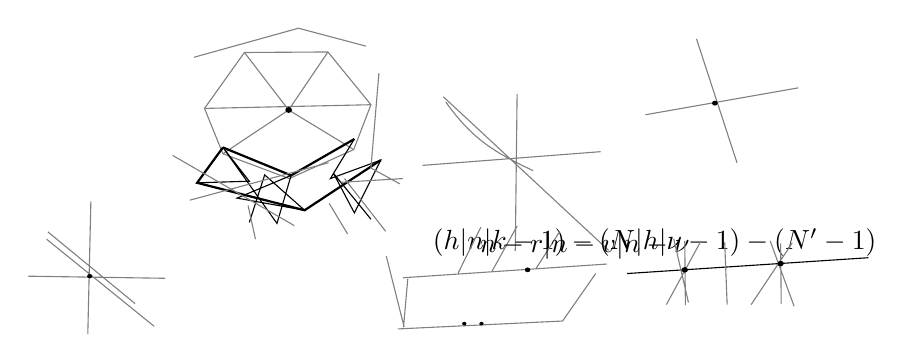
\begin{tikzpicture}[x=.78cm,y=.67cm]
\draw[gray] (1.3,2.55)--(3,3.1)--(4.1,2.76) (1.47,1.58)--(2.12,2.64)--(3.48,2.65)--(4.18,1.65)--(3.9,.8)--(2.85,.25)--(1.77,.72)--cycle;
\draw[gray] (2.12,2.64)--(2.84,1.55)--(3.48,2.65) (1.47,1.58)--(4.18,1.65) (1.77,.72)--(2.84,1.55)--(3.9,.8);
\fill (2.84,1.55) circle (.055);
\draw[thick] (1.77,.84)--(2.88,.31)--(3.91,1.0) (1.77,.84)--(1.35,.17)--(3.10,-.35)--(4.34,.6);
\draw (1.35,.17)--(2.20,.20)--(1.77,.84)--(2.65,-.6)--(2.88,.31)--(2.0,-.12)--(3.10,-.35)--(2.45,.32)--(2.2,-.58) (3.91,1.0)--(3.52,.25)--(4.34,.6)--(3.91,-.4)--(3.57,.35)--(4.18,-.52);
\draw[thin,gray] (.95,.69)--(2.93,-.64) (1.23,-.16)--(3.49,.55) (2.30,-.9)--(2.18,-.26) (3.8,-.8)--(3.5,-.22) (3.75,.25)--(4.42,-.75) (4.31,2.25)--(4.18,.45)--(4.65,.15) (3.7,.18)--(4.7,.25);
\draw[gray] (-1.1,-.9)--(.65,-2.55) (-.43,-2.7)--(-.38,-.18) (-1.4,-1.6)--(.83,-1.64) (-1.08,-.76)--(.34,-2.12);\fill(-.4,-1.6) circle(.042);
\draw[gray] (5.36,1.8)--(8.05,-1.11) (6.56,1.85)--(6.53,-1.12) (5.02,.5)--(7.92,.76) (5.4,1.7)..controls(5.84,.98)and(6.21,.74)..(6.82,.4);
\draw[gray] (8.65,1.46)--(11.14,1.97) (9.48,2.9)--(10.14,.55);\fill(9.78,1.68) circle(.047);
\node at (8.8,-.97) {\handwritten{$(\unsure{h|n|k}-1)-(\unsure{N|h|\nu}-1)-(N'-1)$}};
\draw[gray] (4.62,-2.6)--(7.3,-2.45)--(7.84,-1.55) (4.72,-2.56)--(4.43,-1.22) (4.71,-2.57)--(4.78,-1.65) (4.7,-1.63)--(8.02,-1.37) (5.6,-1.54)--(5.97,-.67) (6.15,-1.51)--(6.56,-.65) (6.86,-1.47)--(7.25,-.76);
\fill(6.73,-1.48) circle(.045);\fill(5.7,-2.5) circle(.035);\fill(5.98,-2.5) circle(.035);
\node at (7.66,-1.02) {\handwritten{$\unsure{n-r|n-v|n-\nu}$}};
\draw (8.35,-1.55)--(12.28,-1.25);\draw[gray] (9.11,-.89)--(9.35,-2.1) (8.99,-2.14)--(9.55,-.94) (9.30,-2.15)--(9.29,-.93) (9.94,-.96)--(9.98,-2.14) (10.37,-2.14)--(11.04,-.97) (10.68,-.93)--(11.07,-2.17) (10.86,-2.12)--(10.85,-.98);
\fill(9.29,-1.48) circle(.052);\fill(10.85,-1.36) circle(.052);
\end{tikzpicture}}
